\section{Results}\label{sec:results}

% Every table below is generated by evaluation/tables.py and every figure by evaluation/figures.py from
% evaluation/analysis/ (evaluation/stats.py); numbers quoted in the prose must be copied from those files after the
% final run (205 configurations, after the Fix 25-27 re-runs).

This section reports the six benchmark dimensions for the human-written and LLM-generated configurations, organised by research question. Unless stated otherwise, figures are medians with interquartile ranges for continuous metrics and proportions with 95\% Wilson intervals for binary outcomes; the statistical tests are those of Section~\ref{sec:method-analysis}, with Holm-adjusted $p$-values.

\subsection{RQ1: LLM-generated versus human-written configurations}\label{sec:res-rq1}

Table~\ref{tab:overview-neutral} and Figure~\ref{fig:dimensions-neutral} compare the neutral-prompt configurations of each model with the manifests the projects ship.

% generated by evaluation/tables.py -- do not edit
\begin{table*}[t]
\centering\small
\caption{Six-dimension results, neutral prompt. Binary rows: percentage (count/n); continuous rows: median [interquartile range]. The human column is the shipped manifest of each project (one per project). D5 time to Ready and D6 are conditional on deployment.}\label{tab:overview-neutral}
\begin{tabular}{lrrrrr}
\toprule
Metric & Human & Claude & DeepSeek & Gemini & Qwen \\ \midrule
Configurations & 7 & 18 & 15 & 15 & 12 \\ \midrule
D1 all objects API-accepted & 100 (7/7) & 100 (18/18) & 100 (15/15) & 87 (13/15) & 67 (8/12) \\
D2 passes PSS baseline & 100 (7/7) & 83 (15/18) & 80 (12/15) & 77 (10/13) & 100 (12/12) \\
D2 passes PSS restricted & 0 (0/7) & 6 (1/18) & 0 (0/15) & 0 (0/13) & 8 (1/12) \\
D2 hard-coded secret & 43 (3/7) & 50 (9/18) & 60 (9/15) & 69 (9/13) & 75 (9/12) \\
D5 fully Ready & 100 (7/7) & 83 (15/18) & 67 (10/15) & 67 (10/15) & 75 (9/12) \\
D5 smoke test passes & 86 (6/7) & 89 (16/18) & 73 (11/15) & 87 (13/15) & 58 (7/12) \\
D6 recovers from all 6 faults & 100 (7/7) & 100 (16/16) & 100 (12/12) & 100 (13/13) & 100 (9/9) \\
\midrule
D2 Kubescape compliance (\%) & 75.0 [73.0, 76.6] & 76.7 [76.5, 77.8] & 75.3 [70.0, 77.9] & 73.3 [72.4, 76.7] & 70.0 [70.0, 72.0] \\
D3 reliability checklist (\%) & 30.7 [20.0, 40.0] & 49.6 [40.1, 53.2] & 25.0 [21.6, 47.5] & 20.0 [16.0, 40.0] & 22.0 [15.1, 30.0] \\
D3 smells per KLOC & 36.0 [23.1, 47.5] & 31.8 [22.2, 37.1] & 39.6 [23.6, 67.8] & 44.8 [39.0, 64.2] & 73.4 [39.8, 76.0] \\
D4 requirements met (\%) & 100.0 [95.8, 100.0] & 100.0 [92.3, 100.0] & 96.3 [91.7, 100.0] & 92.3 [91.7, 96.3] & 100.0 [95.3, 100.0] \\
D5 time to Ready (s) & 20.1 [14.6, 64.0] & 24.8 [11.4, 35.5] & 17.4 [15.3, 19.1] & 13.1 [9.2, 20.3] & 16.8 [12.0, 26.2] \\
D6 availability under faults (\%) & 30.8 [23.2, 64.6] & 53.4 [34.0, 71.0] & 46.4 [33.4, 54.4] & 50.7 [31.8, 63.8] & 45.4 [41.4, 70.1] \\
\bottomrule
\end{tabular}
\end{table*}


\begin{figure*}[t]
\centering
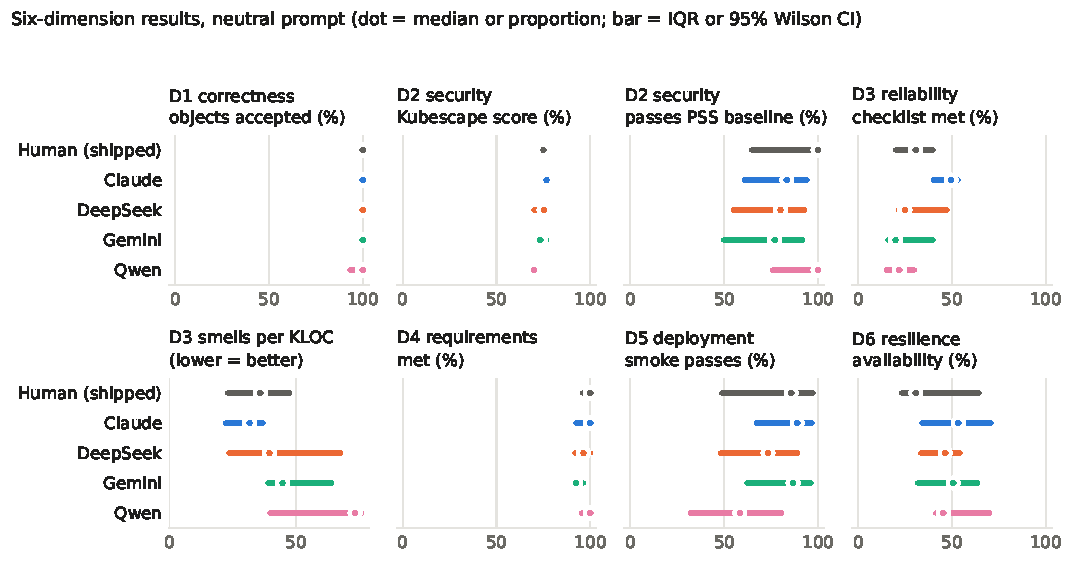
\includegraphics[width=\textwidth]{figures/fig_dimensions_neutral.pdf}
\caption{Six-dimension results for the neutral prompt, one row per source. Dots are medians (continuous metrics) or proportions (binary metrics); bars are interquartile ranges or 95\% Wilson intervals.}
\label{fig:dimensions-neutral}
\end{figure*}

\textbf{Correctness (D1).} Every human manifest and every neutral-prompt configuration from Claude, DeepSeek and GPT was accepted object by object by the API server. Gemini lost two of its 21 configurations, both for the Kubernetes Dashboard, because the provider withheld the response for reproducing training data too closely, and Qwen had all objects accepted in only 10 of its 15 configurations, mostly because it declared Services with several unnamed ports, which a schema validator accepts but the API server rejects. The share of objects accepted differs across sources (Kruskal-Wallis $H=21.81$, $p<0.001$) only because of Qwen (Dunn tests, Holm-adjusted, $p\le0.049$ against the human manifests, Claude, DeepSeek and GPT).

\textbf{Security (D2).} Under the neutral prompt, the generated configurations are about as secure, by static measures, as the manifests the projects ship. Median Kubescape compliance is 76.7\% for Claude, DeepSeek and Gemini, 79.8\% for GPT and 70.0\% for Qwen, against 75.0\% for the human manifests ($H=24.50$, $p<0.001$). GPT (Cliff's $\delta=+0.56$, large) and Claude ($\delta=+0.33$, small) lie above the human manifests and Qwen ($\delta=-0.64$, large) below them, but no pairwise difference with the human manifests survives the Holm adjustment; the significant pairs are Claude--Qwen and GPT--Qwen. Almost nothing reaches the \texttt{restricted} Pod Security Standard (0 of 7 human manifests; 0--24\% of each model's configurations), while 84--100\% of every source passes \texttt{baseline}. A hard-coded secret appears in 43\% of the human manifests and in 52--64\% of each model's configurations, a difference that is not significant ($\chi^2=1.08$, $p=0.956$).

\textbf{Static reliability (D3).} The generated configurations cover more of the reliability checklist than the shipped manifests: the median is 50.0\% for Claude and 54.0\% for GPT against 30.7\% for the human manifests ($\delta=+0.50$ and $+0.72$, both large), and the GPT--human difference is significant after adjustment ($p=0.040$). Gemini (40.0\%), DeepSeek (44.9\%) and Qwen (24.5\%) are close to the human level. KubeLinter smell density does not differ significantly between sources ($H=9.62$, $p=0.087$).

\textbf{Requirements (D4).} Requirement satisfaction is high for every source (medians 96--100\%) and does not differ significantly ($H=10.47$, $p=0.063$).

\textbf{Deployment (D5) and recovery (D6).} Every human manifest became fully Ready and six of the seven passed their smoke test; the exception, Sock Shop, became Ready but its front end no longer served the catalogue, because an image tag the manifest leaves unpinned has since moved. The models' neutral-prompt configurations became fully Ready in 60\% (Qwen) to 86\% (Claude) of cases and passed the smoke test in 47\% (Qwen) to 90\% (Claude). Neither rate differs significantly from the human manifests in any pairwise comparison (Fisher's exact test, all $p\ge0.60$), although seven human configurations give these tests little power. Time to Ready does not differ ($H=5.84$, $p=0.322$). Among configurations that reached fault injection, all recovered from all six injected faults except one GPT configuration; mean availability during the faults (median 30.8\% for the human manifests and 38--45\% per model) and mean recovery time (7.8~s and 13--17~s) do not differ significantly ($H=2.24$, $p=0.815$ and $H=1.77$, $p=0.880$). Restricting D6 to fully Ready configurations changes none of these results.
\textbf{Robustness.} Restricting the comparison to the five projects every model completed changes none of these conclusions: the Kubescape and checklist differences grow slightly (for GPT, $\delta=+0.76$ and $+0.93$; GPT--human checklist $p=0.010$) and the D1 difference remains confined to Qwen. Averaging the three samples of each project and pairing them with that project's human manifest ($n=7$ pairs per model) leaves only GPT's higher checklist coverage significant (median difference $+16.7$ points, Wilcoxon $p=0.031$); the other differences point the same way, but seven pairs give the test little power. Split by the intent of the human manifest, the two production-oriented manifests (Grafana and the Kubernetes Dashboard) score below most models on Kubescape compliance and checklist coverage, with large effect sizes that do not survive the adjustment for multiple comparisons with only two human configurations; the five demonstration-oriented projects reproduce the overall pattern.
The runtime comparisons are equally unchanged on the five common projects and at project level, where no D5 or D6 difference with the human manifests reaches significance.

\subsection{RQ2: Most frequent misconfigurations}\label{sec:res-rq2}

Table~\ref{tab:rahman} reports, for each source and prompt, the share of configurations exhibiting each of the eleven security misconfiguration categories of Rahman et al.\ \citep{rahman2023k8smisconfig}.

% generated by evaluation/tables.py -- do not edit
\begin{table*}[t]
\centering\small
\caption{Share of configurations (\%) exhibiting each security misconfiguration category of Rahman et al., detected with the rules of their SLI-KUBE tool. N = neutral prompt, P = production prompt.}\label{tab:rahman}
\begin{tabular}{lrrrrrrrrr}
\toprule
Category & Human & Claude N & Claude P & DeepSeek N & DeepSeek P & Gemini N & Gemini P & Qwen N & Qwen P \\ \midrule
Absent resource limit & 100 & 61 & 0 & 67 & 8 & 69 & 23 & 83 & 30 \\
Absent securityContext & 71 & 78 & 0 & 80 & 31 & 92 & 92 & 92 & 90 \\
Activation of hostIPC & 0 & 0 & 0 & 0 & 0 & 0 & 0 & 0 & 0 \\
Activation of hostNetwork & 0 & 0 & 0 & 0 & 0 & 0 & 0 & 0 & 0 \\
Activation of hostPID & 0 & 0 & 0 & 0 & 0 & 0 & 0 & 0 & 0 \\
Capability misuse & 0 & 0 & 0 & 0 & 0 & 0 & 0 & 0 & 0 \\
Docker socket mounting & 0 & 17 & 0 & 20 & 8 & 23 & 23 & 8 & 0 \\
Escalated privileges for child processes & 0 & 0 & 0 & 0 & 0 & 0 & 0 & 0 & 0 \\
Hard-coded secret & 57 & 67 & 60 & 60 & 62 & 69 & 69 & 75 & 80 \\
Insecure HTTP & 0 & 17 & 20 & 20 & 15 & 23 & 23 & 25 & 30 \\
Privileged securityContext & 0 & 0 & 0 & 0 & 0 & 0 & 0 & 0 & 0 \\
\bottomrule
\end{tabular}
\end{table*}


Three categories dominate for every source. A hard-coded secret appears in 57\% of the human manifests and in 64--71\% of each model's configurations under both prompts; an absent security context in 71\% of the human manifests and 76--86\% of neutral-prompt configurations; and an absent resource limit in every human manifest and in 24--79\% of neutral-prompt configurations. The production prompt removes most of the last two (for Claude, from 57\% and 76\% to 0\%; for GPT, from 24\% and 76\% to 5\% and 14\%) but leaves hard-coded secrets unchanged. Insecure HTTP is rare (0--25\%) and absent from the human manifests. Docker socket mounting (7--16\% of neutral configurations) occurs only for Sock Shop, whose bundled Compose file mounts the socket while its human manifest does not (Section~\ref{sec:disc-compose}). Host IPC, network and PID sharing, privileged containers, capability misuse and privilege escalation for child processes never occur. The scanners that detect these categories largely agree: on the five security checks Kubescape and Trivy both implement, Cohen's $\kappa$ is 0.88 overall (0.70--1.00 per check).

Compared with the ChatGPT configurations of 2023 studied by Zhang et al.\ \citep{zhang2024genaismells}, current models produce far fewer of the six KubeLinter smells per thousand lines under the neutral prompt: 7.4--10.7 instances of a writable root filesystem against 22.7, 10.8--16.1 of a container that may run as root against 22.8, 1.8--12.4 of unset CPU or memory requests against 45.5 each, and almost no dangling Services (0--0.2 against 6.7). These densities are close to those of the human manifests (5.9--7.7 for the first four smells), with Qwen the highest of the five models. Because our unit is a whole multi-object configuration and Zhang et al.'s a manifest file, the comparison uses density; the share of configurations with at least one instance is inflated by the larger unit and is not compared.

\subsection{RQ3: Differences between models and consistency}\label{sec:res-rq3}

Under the neutral prompt the models differ significantly in Kubescape compliance ($H=23.39$), checklist coverage ($H=18.94$), Polaris score ($H=19.38$) and the share of objects accepted ($H=19.92$; all $p<0.001$). The differences come almost entirely from Qwen, which scores below Claude and GPT on every one of these metrics, and from GPT's higher checklist coverage than Gemini's. Under the production prompt the models separate much more clearly ($H=60.80$ for Kubescape compliance, $46.91$ for checklist coverage and $49.19$ for Polaris score, all $p<0.001$): Claude and GPT form a top group, DeepSeek a middle one, and Gemini and Qwen a bottom one, with every pairwise difference between the top and bottom groups significant after adjustment. Repeating the analysis on the five projects every model completed reproduces both orderings. Requirement satisfaction does not differ between models under either prompt.

The three samples drawn for each model, project and prompt are most alike for Gemini (median across-sample standard deviation 0 for Kubescape compliance and checklist coverage) and least alike for Qwen (15.8 points for the share of objects accepted and 11.1 for checklist coverage); Claude, DeepSeek and GPT lie in between.
The runtime outcome is much less repeatable than the static scores. All three samples of a cell agree on whether the configuration becomes fully Ready in 86\% of cells for Claude, 71\% for Gemini, 50\% for GPT and Qwen and 43\% for DeepSeek, and agree on the smoke-test outcome in 64--71\% of cells for every model. Between models, deployment success differs little under the neutral prompt, where only the smoke-test rate differs ($\chi^2=10.78$, $p=0.029$; Qwen 47\% against 76--90\% for the others), but clearly under the production prompt (Ready $\chi^2=12.25$, $p=0.016$; smoke test $\chi^2=13.95$, $p=0.007$), where Gemini's configurations pass the smoke test in 90\% of cases and DeepSeek's in 38\%.

\subsection{RQ4: Runtime behaviour and the predictive value of static analysis}\label{sec:res-rq4}

Table~\ref{tab:d5-failures} classifies why LLM-generated configurations failed to become fully Ready. Each class is assigned from the cluster's own record of the failed deployment (container exit codes and reasons, restart counts and warning events), captured before the deployment is torn down.

% generated by evaluation/tables.py -- do not edit
\begin{table}[t]
\centering\small
\caption{Classified reason for LLM-generated configurations that did not become fully Ready (D5), by prompt.}\label{tab:d5-failures}
\begin{tabular}{lrrr}
\toprule
Failure class & Neutral & Production & Total \\ \midrule
CrashLoopBackOff & 9 & 14 & 23 \\
NotReady(probe) & 3 & 7 & 10 \\
ContainerCreating & 1 & 1 & 2 \\
no workloads & 1 & 0 & 1 \\
\bottomrule
\end{tabular}
\end{table}


Of the 198 generated configurations, 180 had every object accepted and were deployed, 128 became fully Ready, 136 passed their smoke test and 118 did both. The two outcomes disagree in 28 configurations. In 18, the application served every smoke-test request while some workload never became Ready (six from Gemini, four each from DeepSeek and Qwen, three from GPT and one from Claude), most often an auxiliary component carried over from the Compose file, such as Sock Shop's load generator. In the other 10, every workload was Ready but the application did not work: in six a Service, RBAC object or NetworkPolicy needed on the request path was rejected or misdirected, in one a placeholder domain was enforced, and in three the cause could not be determined, because diagnostics are captured only for configurations that do not become Ready. Table~\ref{tab:root-causes} assigns a root cause to each of the 81 configurations (80 generated and one human) that were not both fully Ready and passing their smoke test; 51 of the mechanisms are directly visible in the cluster's record, 20 are inferred from the manifest together with the observed status, 6 are supported by a matched contrast and 4 remain undetermined. The most frequent are host-level Compose services that fail while the application works (10), invalid YAML or objects the API server rejects (8), hardening that stops a database (7) and liveness probes that kill slow-starting services (6).

% generated by evaluation/tables.py -- do not edit
\begin{table*}[t]
\centering\small
\caption{Root cause of every configuration that was not both fully Ready and passing its smoke test, by model and prompt (N = neutral, P = production). Obs.\ = cases whose mechanism is directly visible in the cluster's record (exit reason, log lines, events, rejected objects or provider stop reason); the remainder are inferred from the manifest together with the observed status, or, for two mechanisms, supported by a matched contrast.}\label{tab:root-causes}
\begin{tabular}{lrrrrrrrrr}
\toprule
Mechanism & Claude & DeepSeek & Gemini & GPT & Qwen & N & P & Human & Obs. \\ \midrule
\multicolumn{10}{l}{\textit{Hardening blocks the workload}} \\
\quad Capability drop or fixed UID stops the database & 3 & 2 & 0 & 2 & 0 & 0 & 7 & 0 & 3/7 \\
\quad runAsNonRoot on an image whose user cannot be verified & 0 & 1 & 0 & 2 & 0 & 1 & 2 & 0 & 0/3 \\
\quad Service-account token disabled for a component that needs the API & 0 & 0 & 0 & 1 & 0 & 0 & 1 & 0 & 1/1 \\
\quad NetworkPolicy blocks a documented internal route & 1 & 0 & 0 & 1 & 0 & 1 & 1 & 0 & 0/2 \\
\multicolumn{10}{l}{\textit{Probes and resource limits}} \\
\quad Liveness/startup probe kills a slow-starting service & 5 & 0 & 0 & 1 & 0 & 2 & 4 & 0 & 2/6 \\
\quad Memory limit too low (OOMKilled) & 0 & 1 & 0 & 1 & 0 & 1 & 1 & 0 & 2/2 \\
\quad Probe on the wrong port or path & 0 & 3 & 0 & 0 & 0 & 0 & 3 & 0 & 1/3 \\
\quad Probe calls a binary the image does not ship & 0 & 0 & 1 & 0 & 0 & 1 & 0 & 0 & 0/1 \\
\quad HTTP probe on a component without a server & 0 & 0 & 0 & 0 & 4 & 1 & 3 & 0 & 0/4 \\
\multicolumn{10}{l}{\textit{Compose file translated literally}} \\
\quad Host-level Compose services break the application & 0 & 1 & 0 & 0 & 0 & 1 & 0 & 0 & 0/1 \\
\quad Host-level Compose services fail; application works & 1 & 2 & 6 & 1 & 0 & 7 & 3 & 0 & 10/10 \\
\multicolumn{10}{l}{\textit{Wrong values or references}} \\
\quad Service targets the wrong container port & 0 & 0 & 0 & 0 & 1 & 1 & 0 & 0 & 1/1 \\
\quad API server address overridden & 0 & 1 & 0 & 0 & 0 & 0 & 1 & 0 & 0/1 \\
\quad Volume references an undefined Secret & 0 & 1 & 0 & 0 & 0 & 1 & 0 & 0 & 1/1 \\
\quad RBAC does not allow updating the CSRF Secret & 0 & 0 & 0 & 1 & 3 & 2 & 2 & 0 & 0/4 \\
\quad No writable /tmp volume on a distroless image & 0 & 0 & 0 & 0 & 1 & 1 & 0 & 0 & 1/1 \\
\quad Image from a non-existent repository & 0 & 0 & 0 & 0 & 2 & 0 & 2 & 0 & 2/2 \\
\quad Required variable set to an empty value & 0 & 2 & 0 & 1 & 0 & 1 & 2 & 0 & 3/3 \\
\quad Non-existent command-line flag & 0 & 0 & 0 & 3 & 0 & 1 & 2 & 0 & 3/3 \\
\quad Placeholder domain enforced & 0 & 0 & 0 & 1 & 0 & 0 & 1 & 0 & 1/1 \\
\quad Points at a database host that does not exist & 0 & 1 & 0 & 1 & 0 & 1 & 1 & 0 & 2/2 \\
\quad TLS required by the client, not offered by the database & 0 & 1 & 0 & 0 & 0 & 0 & 1 & 0 & 1/1 \\
\multicolumn{10}{l}{\textit{Invalid or missing output}} \\
\quad Invalid YAML or object rejected by the API server & 0 & 1 & 0 & 0 & 7 & 4 & 4 & 0 & 8/8 \\
\quad RBAC object rejected (unquoted resource name) & 0 & 2 & 0 & 0 & 0 & 0 & 2 & 0 & 2/2 \\
\quad Reply ends before the YAML block closes & 0 & 0 & 1 & 0 & 2 & 1 & 2 & 0 & 3/3 \\
\quad Provider withheld the reply (recitation) & 0 & 0 & 3 & 0 & 0 & 2 & 1 & 0 & 3/3 \\
\multicolumn{10}{l}{\textit{Other}} \\
\quad Cause not determined & 0 & 3 & 0 & 1 & 0 & 2 & 2 & 0 & 0/4 \\
\quad Unpinned image tag drifted & 0 & 0 & 0 & 0 & 0 & 0 & 0 & 1 & 1/1 \\
\midrule
Total & 10 & 22 & 11 & 17 & 20 & 32 & 48 & 1 & 51/81 \\
\bottomrule
\end{tabular}
\end{table*}


Static scores are a poor guide to runtime behaviour (all correlations Holm-adjusted, pooled over both prompts). No static security or reliability score is associated with becoming fully Ready; only requirement satisfaction is, weakly ($r_{pb}=+0.21$, $p=0.047$). For the smoke test the associations run the wrong way: configurations with higher Polaris scores ($r_{pb}=-0.29$, $p<0.001$) and higher Kubescape compliance ($-0.23$, $p=0.026$) pass it less often, and those with more KubeLinter smells pass it more often ($+0.28$, $p=0.001$). The only positive association with a runtime measure is between checklist coverage and availability during faults ($\rho=+0.30$, $p=0.003$), which is expected because the checklist rewards replicas and disruption budgets. Because the production prompt raises the static scores and lowers deployment success at the same time (Section~\ref{sec:res-rq5}), part of the negative association reflects the prompt rather than a within-prompt relationship; either way, a higher static score does not indicate a configuration more likely to work.

\subsection{RQ5: Effect of requesting production-ready output}\label{sec:res-rq5}

Figure~\ref{fig:prompt-effect} shows, for each model, how the production prompt moves each headline metric relative to the neutral prompt; Table~\ref{tab:overview-production} gives the production-prompt values.

\begin{figure*}[t]
\centering
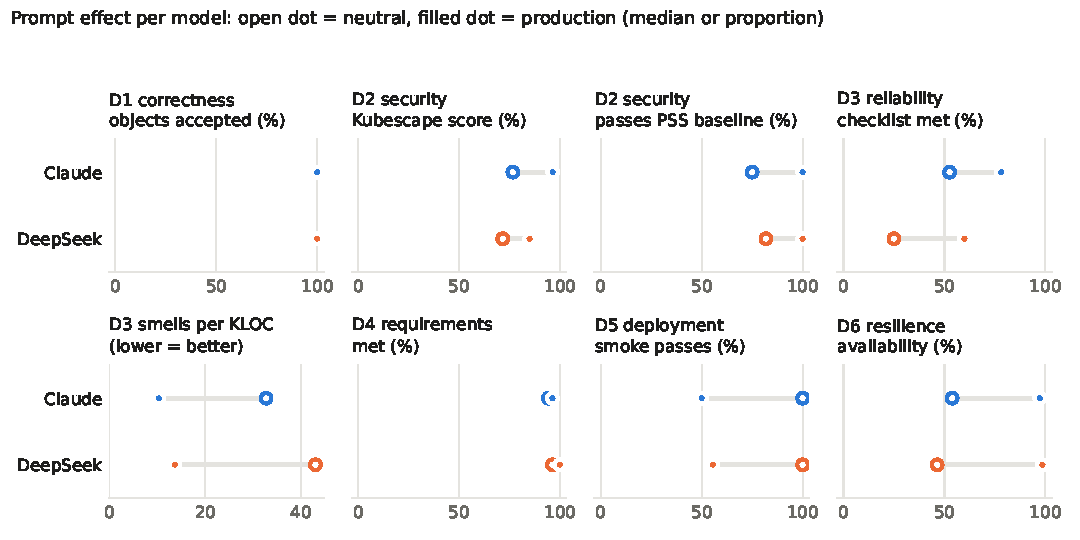
\includegraphics[width=\textwidth]{figures/fig_prompt_effect.pdf}
\caption{Effect of the production prompt per model: open dot = neutral prompt, filled dot = production prompt (median or proportion).}
\label{fig:prompt-effect}
\end{figure*}

% generated by evaluation/tables.py -- do not edit
\begin{table*}[t]
\centering\small
\caption{Six-dimension results, production prompt. Binary rows: percentage (count/n); continuous rows: median [interquartile range]. The human column is the shipped manifest of each project (one per project). D5 time to Ready and D6 are conditional on deployment.}\label{tab:overview-production}
\begin{tabular}{lrrr}
\toprule
Metric & Human & Claude & DeepSeek \\ \midrule
Configurations & 7 & 6 & 11 \\ \midrule
D1 all objects API-accepted & 100 (7/7) & 100 (6/6) & 73 (8/11) \\
D2 passes PSS baseline & 100 (7/7) & 100 (6/6) & 90 (9/10) \\
D2 passes PSS restricted & 0 (0/7) & 17 (1/6) & 20 (2/10) \\
D2 hard-coded secret & 43 (3/7) & 100 (6/6) & 70 (7/10) \\
D5 fully Ready & 100 (7/7) & 33 (2/6) & 36 (4/11) \\
D5 smoke test passes & 86 (6/7) & 33 (2/6) & 36 (4/11) \\
D6 recovers from all 6 faults & 100 (7/7) & 100 (2/2) & 100 (4/4) \\
\midrule
D2 Kubescape compliance (\%) & 75.0 [73.0, 76.6] & 95.9 [92.3, 96.4] & 83.3 [80.0, 86.2] \\
D3 reliability checklist (\%) & 30.7 [20.0, 40.0] & 70.4 [61.3, 79.4] & 59.4 [57.3, 67.7] \\
D3 smells per KLOC & 36.0 [23.1, 47.5] & 10.6 [10.3, 17.6] & 13.7 [7.8, 17.1] \\
D4 requirements met (\%) & 100.0 [95.8, 100.0] & 98.2 [96.3, 100.0] & 98.2 [96.3, 100.0] \\
D5 time to Ready (s) & 20.1 [14.6, 64.0] & 56.4 [55.1, 57.7] & 22.1 [16.2, 27.9] \\
D6 availability under faults (\%) & 30.8 [23.2, 64.6] & 20.4 [20.4, 20.5] & 98.5 [80.1, 99.2] \\
\bottomrule
\end{tabular}
\end{table*}


Asking for production-ready output improves every static measure, for every model. Paired by model, project and sample, median Kubescape compliance rises by 10.0 points ($p<0.001$; significant for each model, from $+3.3$ for Gemini to $+19.8$ for Claude), high and critical Trivy findings fall by 1.5 (by 10 for Claude and 8 for GPT; not significant for Gemini or Qwen), checklist coverage rises by 22.5 points and Polaris score by 13.0 (both significant for every model), and KubeLinter smell density falls by 16.3 per thousand lines (not significant for Gemini). The share of configurations passing the \texttt{restricted} Pod Security Standard rises sharply: 27 configurations pass only under the production prompt and one only under the neutral one (exact McNemar $p<0.001$), led by Claude (11 to 0), DeepSeek and GPT (7 to 0 each). Requirement satisfaction does not change.
Deployment, in contrast, becomes less likely to succeed. Of the configuration pairs whose outcome differs between the prompts, 21 became fully Ready only under the neutral prompt and 5 only under the production prompt (exact McNemar $p=0.002$); for the smoke test the counts are 23 and 7 ($p=0.005$). The loss is spread across Claude, DeepSeek, GPT and Qwen, but is individually significant only for DeepSeek's smoke test (9 against 1, $p=0.021$); Gemini is the exception, with 1 and 2 pairs in each direction. The configurations that do deploy under both prompts are more resilient to faults under the production prompt: median availability during fault injection rises by 9.8 points ($p<0.001$; for Claude by 28.3, $p=0.003$), while recovery time does not change ($p=0.371$) and every configuration that recovered under one prompt also recovered under the other.
